
\textcolor{red}{Are the participants developers? What kind of stakeholders they can be? We can use word stakeholder and define in introduction what we mean by stakeholder: managers, developers, UX etc?}

\section{CROWDED Paradigm}
CROWDEDN where N=0-4 versions will be developed iteratively to help evaluate each version formatively and summatively.

\subsection{CROWDED1 -- Multiple Stakeholder knowledge}
The design of CROWDED1 will be motivated by the cues discovered using CROWDED0 during our empirical investigations. Cues are the cognitive and social weights for the model. Based on our findings, we will create a proof-of-concept CROWDED1 for allowing decision making. 

\subsection{CROWDED2 -- Cloud Knowledge}
CROWDED2, the cues for cloud knowledge (Table 2 will be collected using automatically using a crawler as in our previous studies. The model weights will populate based on model evaluation of cues and fine-tuning them. 

\subsection{CROWD3 -- Verification}

One limitation of the CROWDED 0-2 is that it accept all advice, uncritically. However, humans have fixed and limited attention spans~\cite{davenport2001attention}  which they  have learned to hoard and use sparingly.  
Hence, humans  use heuristic ``short cuts'' that let 
them satisfy the demands of their work, just enough, before rushing off to their next
task~\cite{simon1956rational}.
Such heuristics are essential if humans are to tackle their busy workloads but
can lead to faulty advice. Hence we must ask:

For the purposes of this work, we say
advice is ``faulty'' if it is associated with a bug fixing change, defined as follows.
Suppose we are   exploring
model   for   several days (or longer); e.g.
\bi
\item A team must complete a complex task that requires extensive negotiation;
\item The team is using be reviewing (or updating) old decisions (for auditing or maintenance purposes)
\ei
In this context, there will be two kinds of changes (changes to the models, changes to the advice):
\bi
\item
Changes due to proposed enhancements 
\item
Other changes,  which we would call ``bug fixes''.
CROWDED is 
\underline{\bf faulty} if,      subsequently, it needs   bug fixes.
\ei
We plan to adapt methods from the qualitative and quantitative
literature for automatically generating the fixes, then presented to our stakeholders.

\underline{\em Adapting qualitative methods:}~\cite{Easterbrook08},
it is standard to   take advice from two people 
and, if they cannot agree, then ask a third to resolve the dispute. In this research, we can at least partially automate that ``gang of three'' approach since our $x$ spaces will be annotated with advice from multiple stakeholders.  That is, once faulty advice is found, we can replay the flight of our particles, deleting the influence of the faulty advice.
%then synthesize alternative advice from the landscape around the particle. \textcolor{green}{Not sure if it will work for the tool? Should we remove it?. see comment
 


\underline{\em Adapting quantitative methods:}
co-PI Menzies
has been experimenting with Yu et al.~\cite{yu2019improving}  as follows.  Given a model  executed over an extended period of time,   inputs could be presented to later and older models.
If (e.g.) Wednesday's model
gives different output to Monday's model then that raises a red flag on all the advice from Monday to
Wednesday. As above, we could then replay the flight of the particles, synthesize alternative advice from the landscape around the particle. 
Using delta debugging techniques~\cite{Zeller99}, the difference in the model generated with and without the red flag advice would be something that could be presented to stakeholders for their review. 


 
 
 \subsection{CROWDED 4 --Bias Mitigation}
 
The limitation of CROWDED0-3 is that they do not check for biased advice that 
could lead to the problems of bias and discrimination seen in Table~\ref{tbl:sigh}. 
This is an important issues since, when
    human oversight fails (in the way  discussed by Ben Green in
  \S\ref{why}) then we should
 expect that   software reflects the goals of a few developers (and ignores the concerns of  the wider population).
In that situation, the biases of developers can accidentally and adversely effect the users of that system.  For example, 
 in the case of the COMPAS system discussed in Table~\ref{tbl:sigh} 
 that system was   more likely to falsely label black defendants as future criminals at twice the rate as white defendants.
Hence, we must ask:



% Another example of this effect is offered by Nobel~\cite{noble2018algorithms} who described a hair salon in a traditionally African American neighborhoods that went bankrupt due to bad YELP reviews.  
% Prior to YELP, the  salon successful promoted itself    via word-of-mouth recommendations. But when   YELP become ubiquitous, the   ratings of this business plummeted since its customers made no check-ins from the salon.    
% The owner of this hair salon told Nobel that   that ``Black people don't `check in' and let people know where there at when they sit (in the salon). They already feel like they are being hunted; they aren't going to tell `The Man' where they are.''.   Note that, like the vision system, the designers of the YELP rating scheme were unaware of   social
% differences that effected that rating scheme.

 
 Previously~\cite{Chakraborty_2020,fse21} we have had   success in bias  mitigation
 from machine learning models, measured
 in terms of  (e.g.) reducing the 
  difference in the false positive between African Americans and other social groupings in
 the COMPAS model~\cite{Machine_Bias}. The rest of this section proposes
 adapting and extending those methods within \ITS{4}.
 
 Two of those methods are (1)~{\em hyperparameter optimization}
 and (2)~{\em sample balancing}. While useful,  both these methods have
         a problem with ``in-the-box'' reasoning (described below).
         Hence we also propose evaluating something  new for
  \ITS{4}; i.e.  (3) {\em reasoning  out-of-the-box}. 
 
 Before describing these three methods, we offer two clarifications.  
 Firstly, in \ITS{4}, we would use these approaches at   different times:
 \be
 \item {\em Hyperparameter optimization} runs {\em near the end} of PSO, offering tweaks on   decisions made up to that point;
 \item {\em Sample balancing} runs {\em alongside} PSO, 
 nudging the particles to different places;
 \item  {\em Reasoning out-of-the-box}   runs {\em before} PSO to  change the shape
 of the problem explored by PSO.
 \ee
Secondly,    the following methods can only {\em mitigate}, but may not  {\em remove}, bias.
As stated by  Nobel~\cite{noble2018algorithms} and   Gebru~\cite{gebru21} 
(and many other writers, dating back at least to Crenshaw~\cite{crenshaw2017race}), the root cause of decision
bias is to be found in the social and political structures that select tools favoring small groups within
society. A complete fix for bias   needs to look
at how we select the goals of a system, the designers of that system, and how those designers   go about listening to the people
who use those systems. 

That said, we take   inspiration from Freeman Dyson who   said
{\em technology without morality is barbarous; morality without technology is impotent}. We agree with Dyson: 
if 
we are going to address issues of bias at a very large scale, then we will need some kind of automation to scale that reasoning (e.g. tools like \ITS{4}). More specifically, we seek is a ``two-way street'' between what we might call the {\em humanities view} (which is light on CS knowledge) and the {\em computer science view} (which is light on knowledge of the broader social context). For example, 
Gebru~\cite{adams21a}
wants regulation that ``specifically says that corporations need to show that their technologies are not harmful before they deploy them''.
Implementing that   oversight, at a company-wide scale, would
require many things including tools like what we propose for \ITS{4}; i.e.
(1)~{\em hyperparameter optimization} ,  (2)~{\em sample balancing} 
and (3)~{\em reasoning out-of-the-box}.
  

\noindent\underline{\bf 1. Hyperparameter Optimization (HPO)}: 
 There are many choices in how a machine learner makes a model.
 {\em Hyperparameter optimizers} are automatic tools that can    find options that 
 improve predictive
 performance. Also, as we showed in our FSE'20 paper~\cite{Chakraborty_2020},
 that     process can also be used to select for   models with
 disparities such as those reported for COMPAS.

 Recently, co-PI Menzies    Lustosa~\cite{lustosa22}   explored HPO using {\ITT}.  
 In the work, humans were replaced with a simple oracle that just agreed with whatever decision was ranked most important by {\ITT}. 
 They found that {\ITT} out-performed state-of-the-art HPO tools 
 (FLASH and HYPEROPT and OPTUNA~\cite{bergstra2015hyperopt,nair18,akiba2019optuna}). 
 Accordingly,  for \ITS{4}, we would
   revisit that FSE'20 work to  find even better HPO that remove even more disparity between social groupings. 

  
 
\noindent\underline{\bf 2. Sample Balancing}: 
  When bias arises from an imbalanced
  sampling of   social groupings, then bias can be mitigated by
  adjusting the ratios of those   groupings within the sample
  used to build a model.
  At  FSE'21 co-PI Menzies
 and his student  Joymallya Chakraborty earned a distinguished paper award~\cite{fse21} 
 for a system that extrapolated examples within under-represented social groups within the training data\footnote{Implementation note: that system adjusted frequencies in the 
 {\em training} data and {\bf NOT} the {\em test} data.}.
  Prior to that work, it was  feared   that repairing bias also meant damaging predictive efficacy\footnote{
In 2017,    Berk et al.~\cite{berk2017fairness}   said
"It is impossible to achieve fairness and high performance simultaneously (except in trivial cases".}
But at FSE'21, we    showed that it was   possible to maintain predictive prowess while, at the same time,  reduce bias.

Sample balancing could also be applied to \ITS{4}.
We discussed above methods for {\IT}'s PSO 
 particles to to take advice
 on where they should travel too next. Our FSE'21  data balancing operators 
 from  Menzies and Chakraborty could also be applied to select better directions
 our PSO particles.

   

\noindent\underline{\bf 3. Reasonong Out-of-the-Box}: 
While promising initial steps, {\em hyperparameter optimization}
 and {\em sample balancing}   have   a drawback: they can only reason about  options   found ``in the box'' (i.e. within the current terms and goals of the model).
 This is an incomplete approach since bias can come from things {\em not considered} in the current mode.  For  example,
 Nobel~\cite{noble2018algorithms}   describes a hair salon in a   African American neighborhood that went bankrupt due to bad YELP reviews.  
Prior to YELP, the  salon successful promoted itself    via word-of-mouth recommendations. But when   YELP become ubiquitous, the   ratings of this business plummeted since its customers made no check-ins from the salon.    
The owner of this hair salon told Nobel that   that ``Black people don't `check in' and let people know where there at when they sit (in the salon). They already feel like they are being hunted; they aren't going to tell `The Man' where they are.''.   Note that the designers of the YELP rating scheme guilty of ``in the box'' reasoning since they
did not reflect on how their rating system would work for diverse social groups.

 

Nobel~\cite{noble2018algorithms} and Gebru~\cite{gebru21} claim that systems can become
less biased when their design is effected by a more diverse range of opinions.
In the following, we will test the Nobel/Gebru hypothesis.


\subsection{Interface Design}
The design space for CROWDED interface will be iteratively improved based on evaluation from multiple stakeholders of various expertise (novice and professionals) and gender.

\begin{wrapfigure}{r}{4in}
  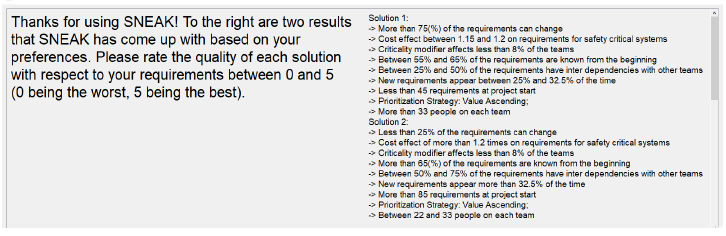
\includegraphics[width=4in]{fig/SNEAK-Interface.png}
\caption{Simple Interface as used in \cite{lustosa21}. 
} \label{sneak}
\end{wrapfigure} 

The initial version of CROWDED was simple (refer Figure \ref{sneak}) and motivated from Cohen's advise in  his book ``Empirical AI'' ~\cite{Cohen95} that it is prudent to compare supposedly sophisticated algorithms against a simpler ``straw system''. For our ``straw'', we would offer humans a simpler browser to a simple GUI showing the models and arcs in our feature models (plus a search box so users can find specific terms) during the CROWDED1-3 versions  to focus on the empirical evaluations. Apart from that simple GUI, we would  offer humans a range of tools that offer advice on what variables are most/least impactful inside a model (and humans will be free to accept, or ignore that guidance).

Final version or deployment version will be provided with sophisticated interface that allows explain the decisions of the CROWDED. Further, it will also give suggestions based on CLOUD and CROWD during decision-making process of humans. The explanation and suggestions  will follow Shneiderman's guidelines \cite{Shneiderman1982} and Neilsen's heuristics  \cite{Nielsen1990}. Furthermore, since the literature \cite{Kuttal2019, Lott2021} indicates gender differences in communication, more comprehensive gender-inclusive language  \cite{festante2007, miller2001handbook} is needed to prepare suggestions to engage, provide non-authoritative suggestions \cite{Seymour2017}. In order to generate accurate suggestions, we may need to consider cues from both study participants as well as cloud.  Gender biases will be eliminated in the CROWDED design using GenderMag \cite{Guizani, Chatterjee}, which helps find and fix gender-related issues in problem-solving software and increase gender inclusiveness. 

We plan to collect and improve interface design based on our lab research and classroom experiences, and contributions from other academics and students via our website.  Also, a CROWDED website will be created for experts to add suggestions to improve the design.

\section{User Studies}\label{rqs}
Extensive lab and case studies will provide data for training, modeling, and evaluating CROWDED functionality and performance.

\subsection{Lab Studies}\label{LabStudy}
Lab studies will be conducted to understand developers' decisions in controlled environments. In addition, small-scale lab studies will be conducted for pilot purposes and to obtain interim evaluation data on small changes to design features and components of CROWDED. The lab study designs and variables are expected to change based on our findings. Each lab study will have the following three key components:

\textbf{Participants} The studies will engage developers with varying expertise. They will be gender-balanced because evaluations of bias in AI tools have found that gender-balanced data in machine learning is crucial to prevent algorithms from perpetuating ideologies that disadvantage women \cite{Leavy2018}. Additionally, our case studies may not provide adequate gender-balanced data due to computer science demographics. We plan to recruit students and professional developers (details in budget). A diverse population of developers will also increase rigor via degrees of freedom \cite{Sjazberg2003}. We will conduct multiple lab studies to bolster confidence in the results. To allow more gender and expert diversity we will conduct virtual lab studies. The virtual lab studies will recruit participants via snowball sampling, advertisements on social platforms, and recruitment websites such as Upwork.

\textbf{Methodology} The think-aloud method \cite{lewisusing, Seaman1999} will be used. Participants will be asked to vocalize their thoughts and feelings as they perform their tasks. We will get individuals as well as teams of developers to complete decision making tasks. Example tasks include: (1) Review a model looking for some bugs (which we would introduce prior that experiment). (2) Modify a model to handle some new requirements. (3) Make decisions within a model in order to optimize the outputs. The participants in the control group will perform tasks using appropriate state-of-the-art optimizers suitable for comparison with automated version of CROWDED. Based on our literature review~\cite{lustosa21} (as of 2021) FLASH and HYPEROPT and OPTUNA~\cite{bergstra2015hyperopt,nair18,akiba2019optuna} will be utilized. These tools allow  human-in-the-loop analysis. The experimental task will include iterations of CROWDED.

As in our past qualitative analyses, we will triangulate (compare and attempt to refute) the results with interviews and surveys to understand their strengths. Retrospective interviews will be conducted to gain insights into participants' experiences and barriers encountered during decision making with and without CROWDED. We will collect: (1) Pre-surveys with standard questionnaires to collect demographics and familiarity with the domain of the model. (2) Pre- and post-surveys with standard questionnaires will be used to evaluate self-efficacy. (3) Post-surveys will be used to analyze the cognitive load using NASA Task Load Index (TLX) to measure and conduct a subjective mental workload (MWL) assessment. 

\textbf{Data Analysis} Video data, audio data and screen interactions of developers will be collected as transcripts, which will be analyzed using a mix of qualitative and quantitative measures. Qualitative methods from Grounded Theory \cite{GlaStr67} (e.g., Corbin and Strauss variant \cite{strauss_basics_1998}) will be used to analyze the transcripts. Central to qualitative analysis is coding the data – identifying points in the data where certain concepts/phenomena are apparent and marking them. We will annotate points based on developer utterances to identify key concepts and phenomena via an iterative, open-coding process, especially for artifact or experience-based cues when making decisions. The cues will be utilized to identify the weights of the model. This process will also be used to analyze decision making behavior. The most common and effective weights will be identified statistically by labeling the outcomes and performing predictive analysis. Finally, thematic analysis \cite{Braun2006} will be used to organize qualitative data into themes that relate back to the research questions.  The Wilcoxon rank-sum test and t-test will be used for quantitative analysis.

\subsection{Case Studies}
\textbf{Participants} We plan to conduct case studies in uncontrolled classroom settings, one in Co-PI Kuttal Software Engineering course (150-200 students per semester) and the other in Co-PI Menzies course (XX-XX students per semester). We will use Mechanical Turk (MTurk) to recruit participants (>300). MTurk is used extensively by academics as a quick and cheap means of collecting questionnaire data, including software engineering research, from a diverse sample of participants. Given the computer science demographics it will be difficult to ensure gender balance in classroom and online settings; however, we will strive to obtain the balance.

\subsection{Models}
Toronto set. others from product line resaerch

\subsection{Metrics}

Initiatl divergance:

final divergence:

y-goal achievement:

user acceptance:

bias metrics: 

\textbf{Methodology} Each student will complete decision task using the think-aloud method. They will record their decision making sessions. We will conduct surveys on their experiences, knowledge tests and end-of-term student course evaluations. Each professional will complete decision based HIT (Human Intelligence Task) using MTurk followed by surveys on their experiences with CROWDED. HIT will have attention checks. An attention check is a question designed to verify that the respondent is reading questions and responding with care. 


\textbf{Data Analysis} Quantitative measures (such as ANOVA) will be used to analyze the scores on tasks, and self-reported surveys on decision making experiences. 

\section{CROWDED Evaluation}
We will conduct continuous evaluations of CROWDED during its development. The results of these evaluations will guide the evolution of CROWDED.  Each evaluation in the cycle will serve as a summative function for the concepts and implementation, and a formative function for the next versions.

We will explore the following research questions.
\bi
\item RQ1: Is  CROWDED useful? I.e if we accept human advice, does that lead to solutions that satisfy more goals? This will be evaluated by all versions of CROWDED.

\item RQ2: If CROWDED relies too much on human advice, will that lead to suboptimal results? CROWDED1 will evaluate.

\item RQ3: If CROWDED tries to use   advice from too many humans, will this confuse the reasoning such that  no one will be satisfied  with the results. CROWDED2 will evaluate.
\item RQ4: Is CROWDED a training tool? i.e. can we use prior    CROWDED to offer guidance (training, assistance) to newcomers ? CROWDED3 will evaluate.
\item RQ5: Is CROWDED a tool for social justice? I.e.can it be used to change designs in order to empower the disempowered?  Or will CROWDED need the bias mitigation tools. CROWDED4 will evaluate.

\ei

\subsection{Models Evaluations}
We will explore different designs for an iSBSE with the goal of let a \underline{\bf broad}
participants explore \underline{\bf many} models to find \underline{\bf better} solutions with \underline{\bf least} effort that are more \underline{\bf acceptable} to more developers. 

We will compare the performance of many models across to increase the generalizability of CROWDED.
 In our prior work assessing SBSE and iSBSE algorithms~\cite{lustosa21,lustosa22,nair18,Nair2016,jchen19} we have found ready access to  10+ models per paper (on effort estimation, agile project planning, waterfall project planning, various configuration models, etc.) to evaluate our methods. More than that, another way to explore many models is to take an existing model and to mutate it such its size increases (measured in terms of number of nodes),  or its complexity increases (measured in terms of number of constraints per node) or both. We have used such model mutators in prior research~\cite{lustosa21}.
 

    
One practical note: in prior work, we found that the limiting factor for this kind
of evaluation is can we find models that humans feel they can comment on. This
issue will have to be carefully explored as part of this work but, for now, we note
that many   models we can access have concepts that many humans   can comment on. E.G.
\bi
\item For a model describing the organization of software projects,
engineers could comment on:  (a)~how many developers need to work together; or
(b)~how to handle high priority tasks within a tight deadline?
\item For a model for on-line shopping:  (a)~what permissions are best for access to past transactions;
(b)~what regress is needed for shoppers such that accidental or fraudulent purchases can be reversed?
\item For a model for predicting recidivism (i.e. probability of repeating  past criminal behavior),
is the model generating similar false positives from African Americans as for Caucasians?
\ei

We take care to distinguish two kinds 
of   solutions:
 
 {\bf ``Acceptable Solutions''}:
 These solutions are judged on a broader criteria that may not appear in a model. 
For example, cost-effective solutions would be  unacceptable if a social justice
advocate argue that society has a duty of care to expend resources on those-in-need (not matter what the expense).
 
 ``Acceptable'' will be measured by  exit questionnaires were users will be asked to express   approval (or disapproval) of the results of the above process.

Another measure of ``acceptable'' will be to show users solutions  generated from   used,fixed, or updated within these experiments. Lustosa reports a procedure for this~\cite{lustosa21}. Given N method for optimizing a model (e.g. {\ITTT} or the iSBSE procedure from   Araujo et al.~\cite{araujo2017architecture}), Lustosa recommends asking 
subjects to rank pairs of 
optimization decisions
(displayed in a random order,
so participants cannot predict which solution comes from which tool).  Users can declare
that neither result is acceptable, or that
 these two results contain insufficient information to judge ``acceptability''.
 
 
 {\bf ``Better Solutions''}:
 ``Better'' solutions
are judged according
to the terms within a  model.
For example, a model might judge that  
 {\em better}
solutions are more cost-effective  where
``cost'' and ``effect'' and defined
within that model.

While
 ``acceptable'' solutions
  are judged according subjective
criteria from   stakeholders,
in this proposal, we say that 
``better'' solutions   are judged   by the $y$ objective
scores seen when models are run using
the decisions from our stakeholders

There is a rich literature in the SBSE
community on how to judge  ``better''.
For example, the following nodes come
from  Li et al.'s recent
IEEE TSE 2021 paper~\cite{li20}. 
 When working with multiple stakeholders, its prudent to assume that they will
 have many goals, some of which can achieved only by ``trading off'' other goals.
In such a goal space, no single solution may be ``best''. Rather, many solutions will be unacceptable
and the survivors will form a ``Pareto front'' of possibilities. 
More precisely, 
for two solutions $\mathbf{a}, \mathbf{b} \in Z$
($Z \subset \mathbb{R}^m$, where $m$ denotes the number of objectives),
solution $\mathbf{a}$ is said to \textit{weakly dominate} $\mathbf{b}$
(denoted as $\mathbf{a}\preceq \mathbf{b}$)
if $\mathbf{a}_i \leq \mathbf{b}_i$ for $1 \leq i \leq m$.
If there exists at least one objective $j$ on which $\mathbf{a}_j < \mathbf{b}_j$,
we say that $\mathbf{a}$ \textit{dominates} $\mathbf{b}$ (denoted as $\mathbf{a}\prec \mathbf{b}$).
A solution $\mathbf{a} \in Z$ is called \textit{Pareto optimal}
if there is no $\mathbf{b} \in Z$ that dominates $\mathbf{a}$.
 The set of all Pareto optimal solutions of a multi-objective optimization problem is called its \textit{Pareto front}.
Based on their reading of the SE
literature, Table~9 of Li et al.~\cite{li20} lists 12   indicators used to evaluate such Pareto-based
reasoning and note that   in the literature, there is no clear consensus on how to select between these different indicators. Hence,
 Li et al. argue that domain criteria should be used to select
an appropriate indicator. 
For example,
reading their text, it would seem that 
  CI (the {\em contribution indicator}) is most appropriate for our work.
Li et al. comment that  CI is useful when trying to know the relative quality between treatments (e.g. {\ITT} vs {\ITTT}).
CI 
calculates the ratio of the solutions of a set that are not dominated by any solution in the other set. 
Given two sets $\mathbf{A}$ and $\mathbf{B}$ from two treatments:

\begin{small}
	\begin{equation}
	CI(\mathbf{A},\mathbf{B}) = \frac{|\mathbf{A}\cap \mathbf{B}|/2 + |\mathbf{A}_{\prec B}| + |\mathbf{A}_{\npreceq \cap \nsucc B}|}{|\mathbf{A}\cap \mathbf{B}| + |\mathbf{A}_{\prec B}| + |\mathbf{A}_{\npreceq \cap \nsucc B}| + |\mathbf{B}_{\prec A}| + |\mathbf{B}_{\npreceq \cap \nsucc A}|}
	\label{eq:CI}
	\end{equation} 
	\end{small}where $\mathbf{A}_{\prec B}$ are the  solutions in $\mathbf{A}$ that dominate some solution of $\mathbf{B}$ (i.e., $\mathbf{A}_{\prec B} = \{\mathbf{a} \in \mathbf{A}| \exists \mathbf{b} \in \mathbf{B}: \mathbf{a} \prec \mathbf{b}\}$), 
	and $\mathbf{A}_{\npreceq \cap \nsucc B}$ are the solutions in $\mathbf{A}$ that do not weakly dominate any solution in $\mathbf{B}$ and also are not dominated by any solution in $\mathbf{B}$ (i.e., $\mathbf{A}_{\npreceq \cap \nsucc B} = \{\mathbf{a} \in \mathbf{A}| \nexists \mathbf{b} \in \mathbf{B}: \mathbf{a} \preceq \mathbf{b} \vee \mathbf{b} \prec \mathbf{a}\}$). Note that {\em higher} CI values
	are {\em better}.
	

 Having made this separation between
 ``better'' and ``acceptable'',
 we note that it is an open issue
 if users will judge better solutions
 as more acceptable, of vice versa (see
 {\bf RQ3}, beow).
 
 {\bf ``Completion time''}: Given access to teams of people working on numerous models, we can evaluate this work asking different groups to work with different models such as {\ITTT} or traditional iSBSE methods. As said above, we will get teams to modify, debug, or apply a set of models in an environment where they can access a variety of tools, including {\ITTT} and {\ITT}, manual browsing tools, and iSBSE tools from other researchers.  The time to complete tasks will be collected. We will declare {\ITTT} useful if it results in better and more acceptable models, in less time.


\subsection{Cues Collection using CROWDED0}
We will conduct gender and expert-balanced lab studies to collect initial set of cues utilized by the stakeholders when making decisions. Remember cues are the social and cognitive weights of the model that helps to prioritize the decision from different stakeholders. These studies will also help in conducting case studies for class and Mturk. Students in the classes and professional using Mturk tasks will make decisions and will collect the respective cues. The cues collected using lab study and cae studies along with literature-based will help in creating a large scale survey and interviews.
\subsection{CROWDED1: experience based Cues, model evaluation}
CROWDED1 will utilized the expert's experience based cues and will be evaluated using model. 

If the methods of \S\ref{better} {\em do not} change the conclusions reached  by {\IT}, then we would need alternate methods for applying advice from our stakeholders' footprint to our reasoning. Comparing the optimization results achieved without and without the extra cues from Table~\ref{info}. For those comparisons, we will take  guidance from:
\bi
\item Arcuri and Briand~\cite{Arcuri11} on the analysis of stochastic algorithms  (multiple trials;    different random   seeds);
\item Shepperd and  MacDonell~\cite{SHEPPERD2012820}  on augmenting
 non-parametric significance tests with effect size tests;
 \item
 Li et al.   IEEE TSE 2021 paper~\cite{li20} on   appropriate indicators for  multi-objective optimization studies.
 \ei

We also believe that there is some ``negotiation cliff'' after which all the tools described here will fail to find any consensus. The discovery of the location of this negotiation cliff would tell us what are the limits to collaboration over a model. Our belief is that this would  one of the important results     arising from this research.

The   framework   allows to measure both the initial and final disagreement.
To measure the  initial disagreement:
\bi
\item
Take 100 terms are random from the domain.
\item
Submit as input to sentiment tools looking at the electronic footprint of different stakeholders.
\item
Count how often the same term gets the same sentiment from different stakeholders.
\ei
To measure, final agreement, we need to look at the final positions of the particles in the PSO:
\bi
\item If   particles can   find solutions acceptable to most parties, then  they will converge to a few small regions.
\item
 If    stakeholders are implacably opposed, then   particles from converge
 to very different locals in $x$-space.
\ei
We predict that after some threshold value in the initial disagreement, there will be no final convergence. We will compare 

{\tt Evaluation:} Metrics for model evaluation will include: (i) higher accuracy of the model, and (ii) specific negotiation cliffs for the model weights.

\subsection{CROWDED2: cloud based cues, Model evaluation, lab studies}

CROWDED2 will utilize cloud based cues (automatically generated from logs as in Table 2). We will evaluate the model with different weights to evaluate the best weight distribution strategy used by CROWDED2. Based on the finalized model we will use a simple interface to evaluate the model with gender and expert-balanced lab studies. We will collect qualitative and quantitative data.  Qualitative analyses will focus on transcripts and interviews. Quantitative analyses will employ the Wilcoxon rank-sum test or t-tests.

{\tt Evaluation:} The metrics include: (i) student and professional task success; (ii) completion times, (iii) student experiences (e.g., satisfaction and engagement) with CROWDED3 using end-of-term student course evaluations, (iv) accuracy of questionnare score with the model score.

\subsection{CROWED3: Prioritize and feedback generation, Case studies}
CROWDED3 will help with verification. The model will find the possible conflicting advice from the model based on multiple stakeholder's knowledge and utilize automatic fixes. This model will be evaluated by comparing various fixing techniques from literature for specific conflicts. CROWDED3 will be improved with better interface that generate feedback as well as explanations for CROWDED3 advice and decisions.

CROWDED3 will evaluated using Comparative case studies with students and professionals. In class settings students will complete (i) first assignment without CROWDED3; (ii) second assignment with CROWDED3; and (iii) third assignment optionally with CROWDED3.  Similarly, using Mturk participants will complete decision making tasks with and without CROWDED3. Three-way ANOVA and two-way between-subjects tests will be used to measure decision performance and model acceptance. Further, the scores (from the model) will be compared to participants questionnaires. The results will also help assess the usability and generalizability of CROWDED3 in real-world settings. 

{\tt Evaluation:} additional metrics for model evaluation: Based on what we have seen in traditional software analytics, there are two expectations. (i) frequency of the Faulty advice, and (ii) time to fix faults (should have some exponential decay where most are fixed quickly, but a few may take comparatively much longer).

\subsection{CROWED4: Inclusive design, Model Evaluation, lab study}

CROWED4 interface design will be inspired from gender-based research and evaluated with GenderMag (as discussed in Section XX). 

Further, the model will be improved to minimize social biases by including related measures in the PSO optimization goals. The effects of decisions on different social groups can be assessed via (e.g.) reducing the difference in the false positive between African Americans and other social groupings in the COMPAS model~\cite{Machine_Bias}. Recently we completed a literature review~\cite{Majumder21} that found 30 such bias-related metrics which, after   clustering, we could reduce to around half a dozen. This will help in HPO optimization and making model inclusive.

The models generated will be designed to fairer by balancing and will be done similar to HPO. Also, as in our FSE'21 paper~\cite{fse21}, we would also require that these
 fairness improvements do not come at the cost of inference performance.
 
We will utilize different levels of diversity to address the same model maintenance task. An exact measure of initial divergence will be taken using the same ``take 100 terms'' test used in (as discussed before). An initial and final measure of model bias will be taken as described above in HPO. We would have confirmation of the  Nobel/Gebru conjecture if increased team diversity is seen to be associated with greatest decrease in model bias (i.e. final minus initial).

Based on the finalized model we will evaluate CROWDED4 with gender and expert-balanced lab studies. We will collect qualitative and quantitative data.  Qualitative analyses will focus on transcripts and interviews. Quantitative analyses will employ the Wilcoxon rank-sum test or t-tests.

{\tt Evaluation:} additional metrics: (i) gender-based biases, (ii) highest model accuracy with bias-based metrics.

\subsection{CROWED: Final Evaluation, Deployment, Website}
The final version of CROWDED4 will be evaluated using case studies in the class and Mturk. We will collect the data from different race and gender especially in our MTurk studies. The final version of inclusive-CROWDED will be deployed online for industry and universities through a dedicated website. 

{\tt Evaluation:} additional metrics: (i) number of download, (ii) number of views.



\begin{figure*}[t]
\centerline{\includegraphics[width=0.98\textwidth]{fig/PLAN.PNG}}
\caption{3-year plan.}
\label{Overall}
\end{figure*}



\section{Schedule} 


 \begin{wraptable}{r}{3.35in}
{ \footnotesize
\begin{tabular}{|l|l|l|l|}\cline{2-4}    
\multicolumn{1}{c|}{~}      &\multicolumn{3}{c|}{Year} \\
\multicolumn{1}{l|}{~}       &1 & 2 & 3  \\\hline  
{\bf Goal2:} run faster                   &   x  &  &   \\\hline 
{\bf Goal1:} better post-attack performance         &    x  &       &   \\\hline 
{\bf Goal3:} test against adaptive adversaries        &      & x      &   \\\hline  
{\bf Goal4:}  test in numerous domains                &      & x     &       \\ \hline
{\bf Goal5:} inspect the decision boundaries           &      & x      &  x     \\ \hline
BPC work (broadening participation in computing)  &   x &  x    & x     \\ \hline
\end{tabular} } 
\caption{Timetable for this work. }\label{when}
\end{wraptable}
Table~\ref{when} shows a three-year plan from this work.
Note that   will explore {\bf GOAL2} first since, if successful, this will speed up everything else.
Also,  we   explore {\bf GOAL5} last since everything up till
then has the potential to change the generated decision boundaries.

Lastly, 
one  of the benefits of  NSF funding
is the opportunity to work on  broadening participating in computing (BPC).  Our BPC plans are discussed in \S\ref{bpc}. As seen
  in our timetable, BPC will be an on-going task through-out the work.





 
